\documentclass[11pt,aspectratio=169,dvipsnames]{beamer}
\graphicspath{{figs/}}
\usetheme{default}
\usepackage{DasBeamerPaket}
\usepackage{animate}
\usepackage{lastpage}
%\usepackage{enumitem}
\usepackage{appendixnumberbeamer}
\usepackage{braket}
\usepackage{tikz}
\setbeamercolor{section in toc}{fg=NavyBlue}
\setbeamercolor{frametitle}{fg=NavyBlue}
\captionsetup[figure]{labelfont=bf}
\captionsetup[table]{labelfont=bf}
\newcommand{\theauthor}{Jakob Krause}
\newcommand{\theshortauthor}{\textsc{J. Krause} for CBELSA/TAPS}
\newcommand{\authormail}{krause@hiskp.uni-bonn.de}
\newcommand{\authorgit}{krausejm}
\newcommand{\thetitle}{Recent Polarization Observable Results in  $\eta$- and $\eta'$-photoproduction off the proton}
\newcommand{\theshorttitle}{$\Sigma$ in $\eta$- and $\eta'$ photoproduction}
\newcommand{\thecolor}{black!70!blue}
\newcommand{\thecolorr}{black!60!blue}
\newcommand{\thecolorrr}{black!50!blue}
\newcommand{\thesubtitle}{Master thesis for the CBELSA/TAPS collaboration}
\newcommand{\thedate}{30th March 2022}
\makeatletter
\patchcmd{\beamer@calculateheadfoot}{\advance\footheight by 4pt}{\advance\footheight by 20pt}{}{}
\makeatother
\begin{document}
	\definecolor{myWhite}{rgb}{1,1,1}
	
	
	\setbeamercolor{coloredboxstuff}{fg=myWhite,bg=\thecolor}
	\setbeamercolor{coloredboxstuff1}{fg=myWhite,bg=\thecolorr}
	\setbeamercolor{coloredboxstuff2}{fg=myWhite,bg=\thecolorrr}	
	\makeatother
	\setbeamertemplate{footline}
	{
		\leavevmode%
		\hbox{%
			\begin{beamercolorbox}[wd=.33\paperwidth,ht=2.25ex,dp=1ex,center]{coloredboxstuff}%
				{\theshortauthor}
			\end{beamercolorbox}%
			\begin{beamercolorbox}[wd=.34\paperwidth,ht=2.25ex,dp=1ex,center]{coloredboxstuff1}%
				{\theshorttitle}
			\end{beamercolorbox}%
			\begin{beamercolorbox}[wd=.33\paperwidth,ht=2.25ex,dp=1ex,center]{coloredboxstuff}%
				\insertframenumber{} / \inserttotalframenumber\hspace*{1ex}
		\end{beamercolorbox}}%
	}
	\makeatletter
	
	
	\setbeamercovered{transparent}
	\setbeamertemplate{navigation symbols}{}
	\setbeamertemplate{frametitle}[default][left,leftskip=0.5cm]
	\setbeamertemplate{itemize item}{\color{black}$\blacktriangleright$}
	\setbeamertemplate{section in toc}[sections numbered]
	\setbeamercolor{section in toc}{fg=\thecolor}
	\setbeamercolor{frametitle}{fg=\thecolor}
	\captionsetup{font=scriptsize,labelfont=scriptsize}
	\AtBeginSection[]
	{	
		
		{
			
			\makeatother
			\setbeamertemplate{footline}
			{
				\leavevmode%
				\hbox{%
					\begin{beamercolorbox}[wd=.34\paperwidth,ht=2.25ex,dp=1ex,center]{coloredboxstuff}%
						{|\hfill\theshortauthor\hfill|}
					\end{beamercolorbox}%
					\begin{beamercolorbox}[wd=.34\paperwidth,ht=2.25ex,dp=1ex,center]{coloredboxstuff}%
						{\theshorttitle}
					\end{beamercolorbox}%
					\begin{beamercolorbox}[wd=.34\paperwidth,ht=2.25ex,dp=1ex,center]{coloredboxstuff}%
						\insertsection\hspace*{1ex}
				\end{beamercolorbox}}%
			}
			\makeatletter
			
			
			\begin{frame}[noframenumbering]
				\frametitle{}
				\addtocounter{page}{-1}
				\tableofcontents[currentsection]
			\end{frame}
		}
		
	}
	%\begin{frame}[plain]
	%	\centering
	%	{\Large \color{\thecolor}{\thetitle}}\\
	%	\vspace{0.5cm}
	%	{\thesubtitle}
	%	\vfill
	%	\begin{minipage}{\linewidth}
		%		\centering
		%		\begin{minipage}{\linewidth}
			%			\textsc{\theauthor}\\
			%			\scriptsize \href{mailto:\authormail}{\faEnvelope  \hspace*{0.1cm}\authormail} {\color{black}$|$} \href{https://github.com/\authorgit}{\faGithub  \hspace*{0.1cm}\authorgit}\\
			%		\end{minipage}
		%		\vspace{.5cm}
		
		%		{\scriptsize
			%			Supervisor: \textsc{Jun. Prof. Dr. Annika Thiel}\\
			%			\tiny \href{mailto:thiel@hiskp.uni-bonn.de}{\faEnvelope  \hspace*{0.1cm}thiel@hiskp.uni-bonn.de}\par}
		%	\end{minipage}
	%	\vspace{0.2cm}
	
	%	\thedate
	%\end{frame}
	
\begin{frame}{Event based ML fit for $\eta'$ data}
		\begin{tcolorbox}[colback=blue!5,colframe=\thecolor,title=Methods]
			\begin{itemize}
				\item \texttt{TTree::UnbinnedFit()}
				\item \emph{RooFit} (WIP)
				\item event based fit using \textsc{bayesian} inference
				\begin{itemize}
					\item with and without fitting bkg contributions
				\end{itemize}
			\end{itemize}
		\end{tcolorbox}
	each case: no measure of "goodness of fit" $\to$ toy MC necessary (as before)
\end{frame}
\begin{frame}{Remembering PDF to be fitted...}

		\begin{align*}
			-\ln\mathcal{L}=&\sum_{i=1}^{n}-\ln(p_\text{prompt}(\phi_i,p_{\gamma,i},\Sigma,a_1\dots a_4,b_1\dots b_4))+\\
			&\sum_{j=1}^{m}-\ln\left(p_\text{sideband}(\phi_j,p_{\gamma,j},\Sigma^\text{bkg},a_1^\text{bkg}\dots a_4^\text{bkg},b_1^\text{bkg}\dots b_4^\text{bkg})\right)
		\end{align*}
		where
		\begin{align*}
			p_\text{prompt}&=f_{\text{sig}}\cdot\tilde{p}(\phi,p_\gamma,\Sigma,a_1\dots a_4, b_1\dots b_4)\\ &+ \left(1-f_\text{sig}\right)\cdot\tilde{p}(\phi,p_\gamma,\Sigma^\text{bkg},a_1^\text{bkg}\dots a_4^\text{bkg}, b_1^\text{bkg}\dots b_4^\text{bkg})\\
			p_\text{sideband}&=\tilde{p}(\phi,p_\gamma,\Sigma^\text{bkg},a_1^\text{bkg}\dots a_4^\text{bkg}, b_1^\text{bkg}\dots b_4^\text{bkg})
		\end{align*}
		and \begin{equation*}
			\tilde{p}(\phi,\Sigma)=\frac{\left(1+p_\gamma\Sigma\cos\left(2\left(\alpha^\parallel-\phi\right)\right)\right)\cdot\left(\sum_{k=0}^{4}a_k\sin(k\phi)+b_k\cos(k\phi)\right)}{1-\frac{1}{2}a_2p_\gamma\Sigma}
		\end{equation*}

\end{frame}
\begin{frame}{Considering background contributions}
	\begin{itemize}
		\item simulate $\eta'$ statistics and bkg contributions in toy MC
		\item expectation: $\Sigma_\text{meas}=a\cdot\Sigma_\text{true}+b\cdot\Sigma_\text{bkg}$, where $a+b=1$
		\item $\Sigma_\text{true}=0.5,\Sigma_\text{bkg}=-0.3,a=0.8 \to \Sigma_\text{meas} = 0.34 $ 
	\end{itemize}
	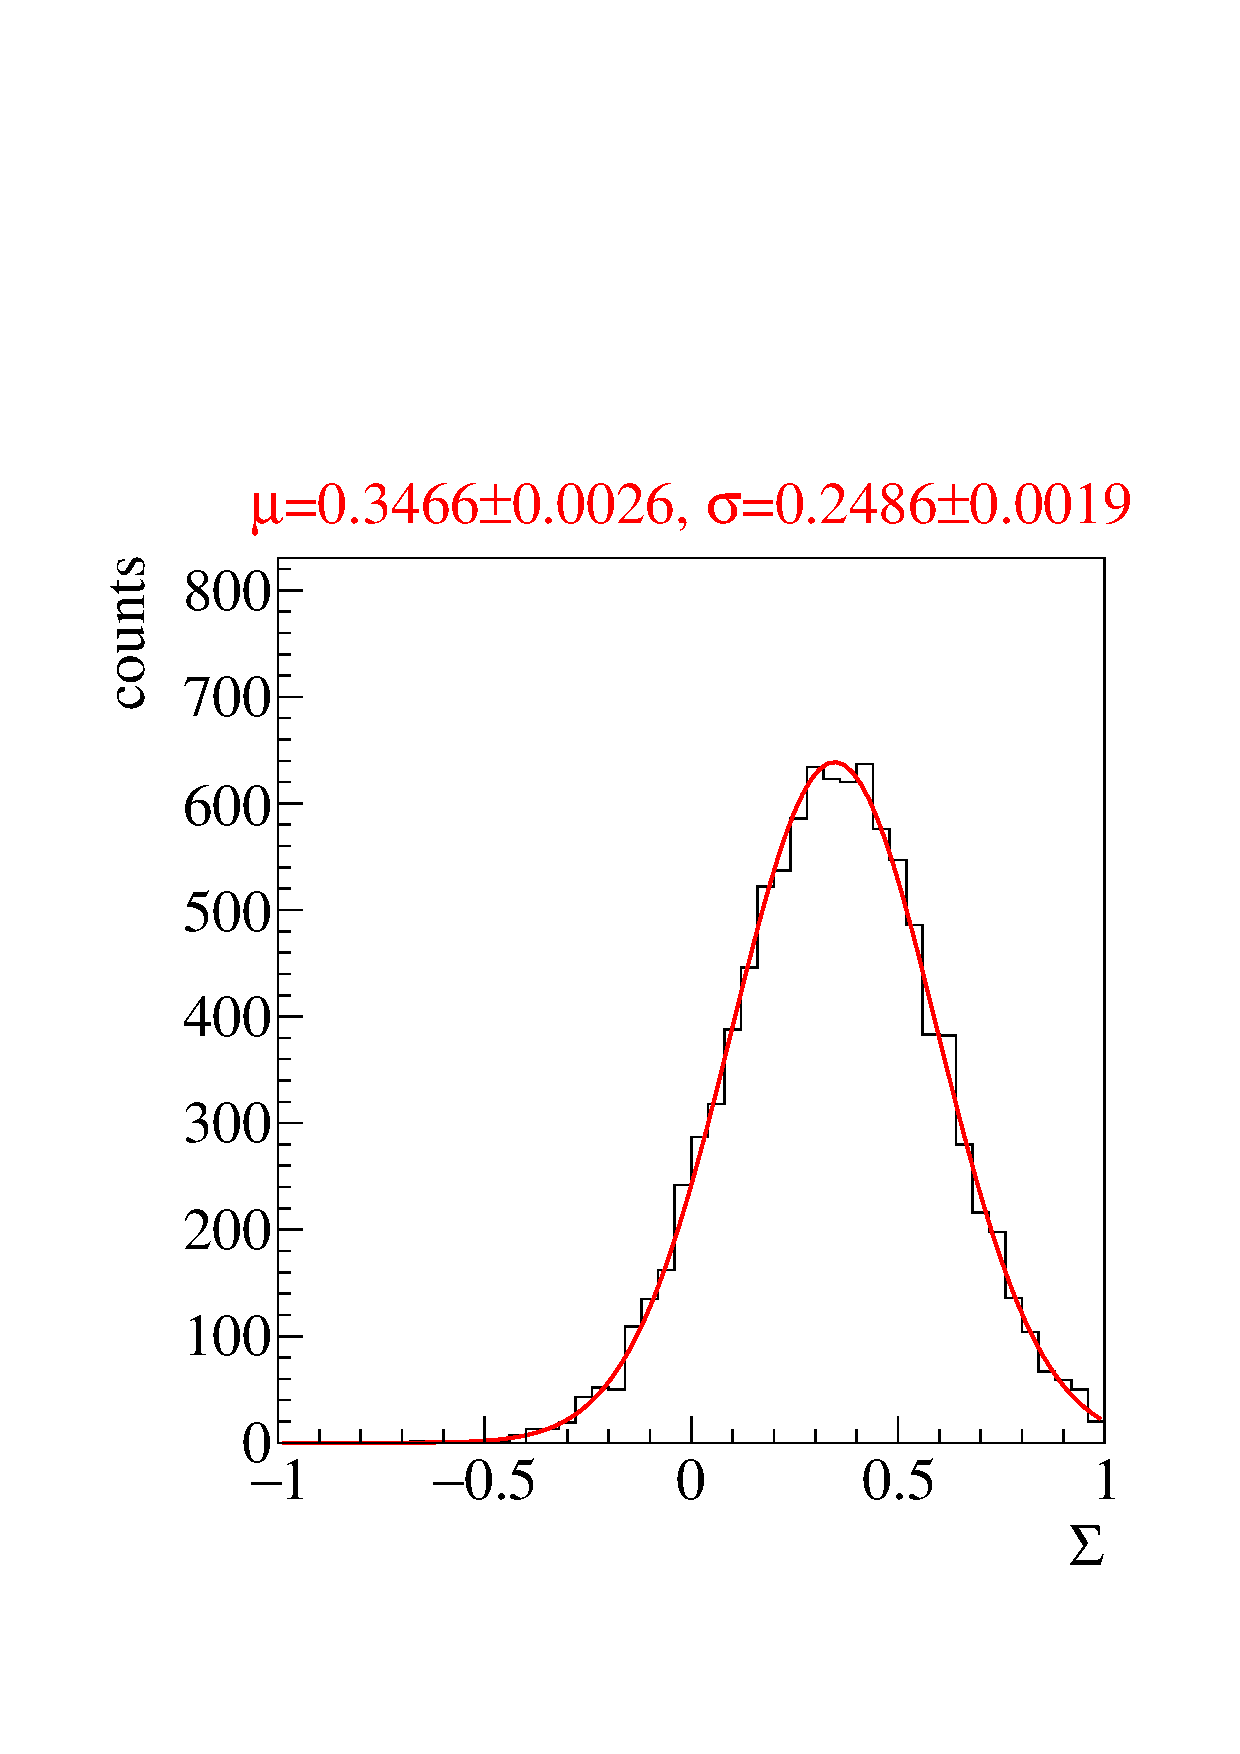
\includegraphics[width=.49\linewidth]{../../RooFit/plots/sigma.pdf}
		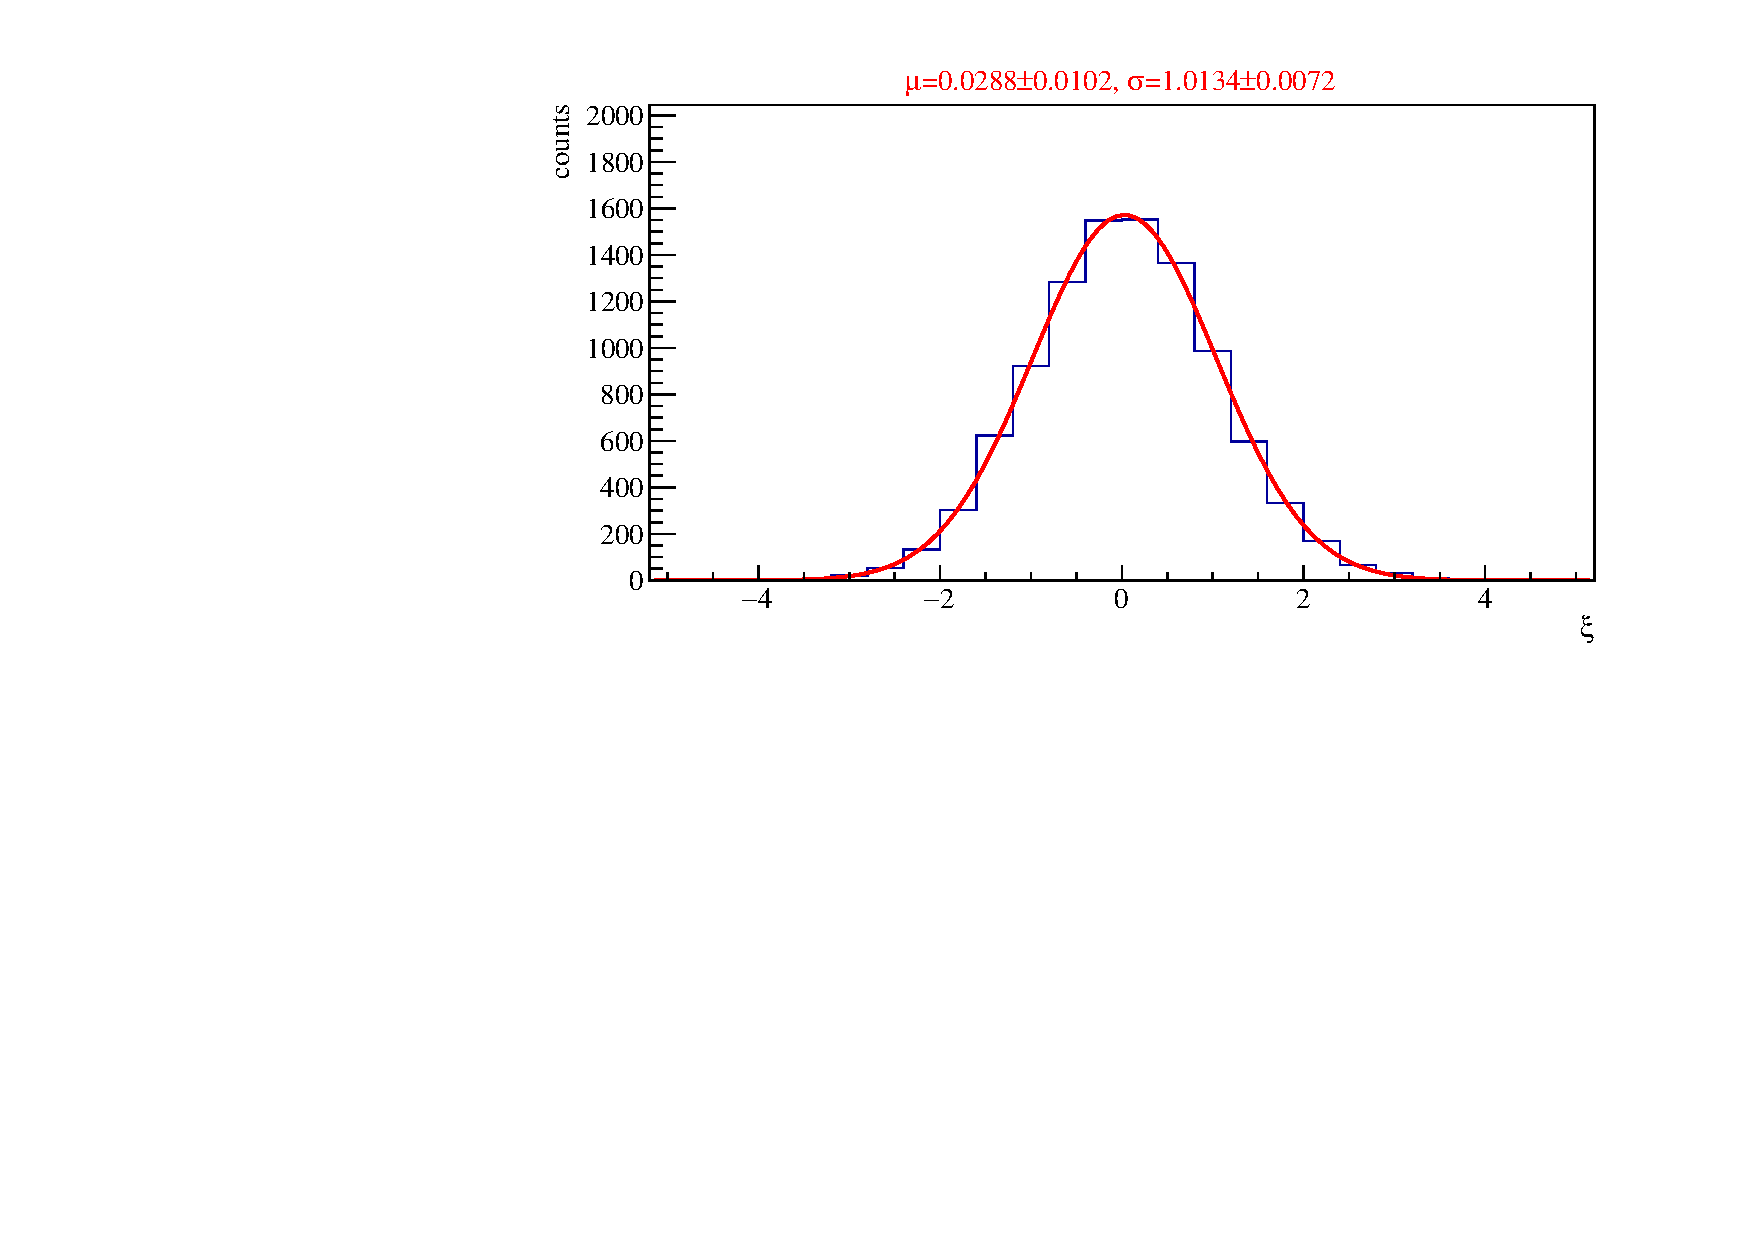
\includegraphics[width=.49\linewidth]{../../RooFit/plots/residuals.pdf}
\end{frame}
\begin{frame}{Considering background contributions}
	\begin{itemize}
	

	\item If background contribution is known, it can directly be included in the \textsc{bayesian} fit by treating it as "missing data"
	\item \begin{equation*}
		\tilde{p}(\phi,\Sigma)=\frac{\left(1+p_\gamma\Sigma\cos\left(2\left(\alpha^\parallel-\phi\right)\right)\right)\cdot\left(\sum_{k=0}^{4}a_k\sin(k\phi)+b_k\cos(k\phi)\right)}{1-\frac{1}{2}a_2p_\gamma\Sigma}
	\end{equation*}
	with $\Sigma=(a\cdot\Sigma_\text{true}+b\cdot\Sigma_\text{bkg}$) and $a,b,\Sigma_\text{bkg}$ are read in as data
	\item statistical error of $\Sigma_\text{bkg}$ can be accounted for by fitting an additional unknown parameter $\Sigma_{\text{bkg}}^{\text{true}}$, assuming $$\Sigma_{\text{bkg}}^{\text{true}}\sim\text{normal}(\Sigma_\text{bkg}^\text{meas},\text{err}(\Sigma_\text{bkg}^\text{meas}))$$ with uniform prior and then using $\Sigma_{\text{bkg}}^{\text{true}}$ as $\Sigma_{\text{bkg}}$ in $p(\phi,\Sigma)$ 
	\end{itemize}
\end{frame}
\begin{frame}{Considering background contributions}
toy MC with same dataset as before (assuming $\text{err}(\Sigma_{\text{bkg}}^\text{meas})=0.05$) reproduces input values very nicely

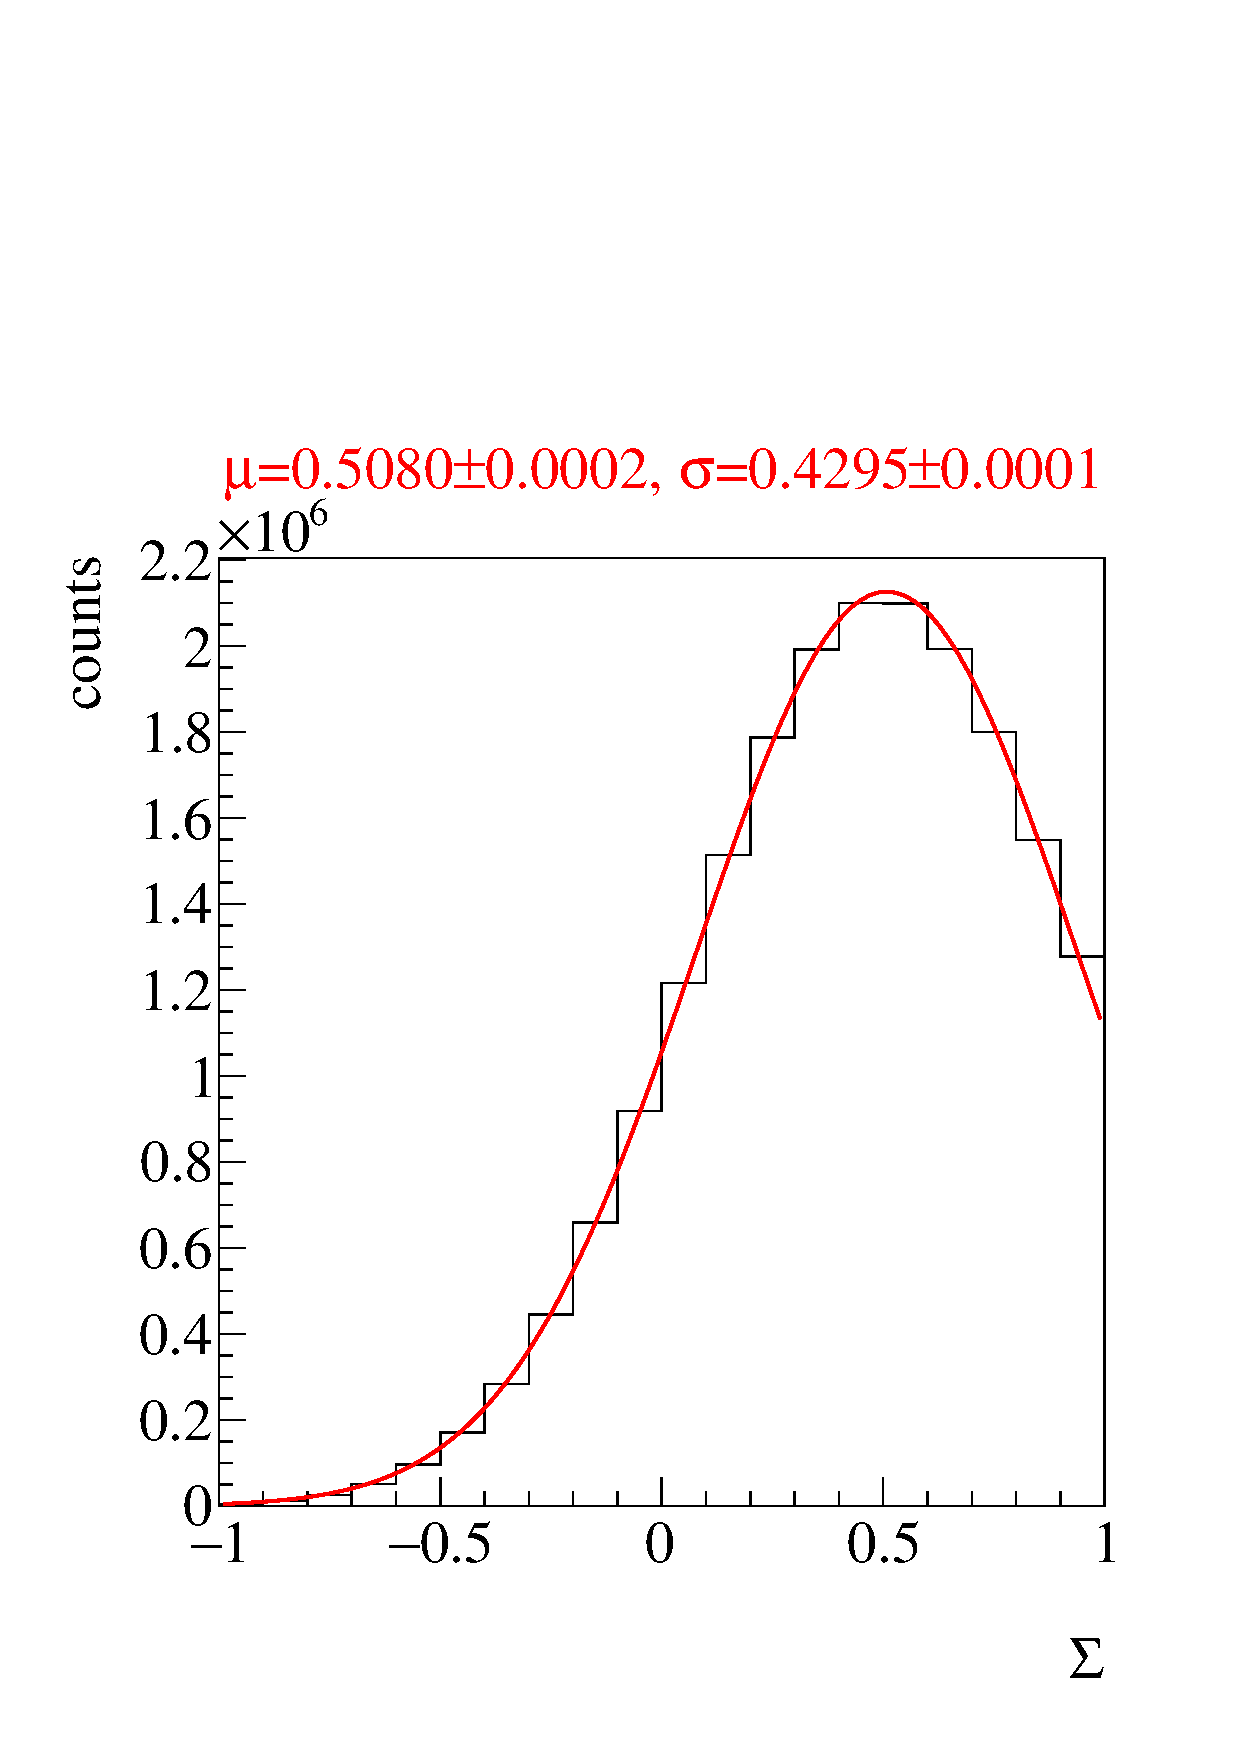
\includegraphics[width=.49\linewidth]{../../bayes/etap_event_based_fit/plots/combined_post_add_raw.pdf}
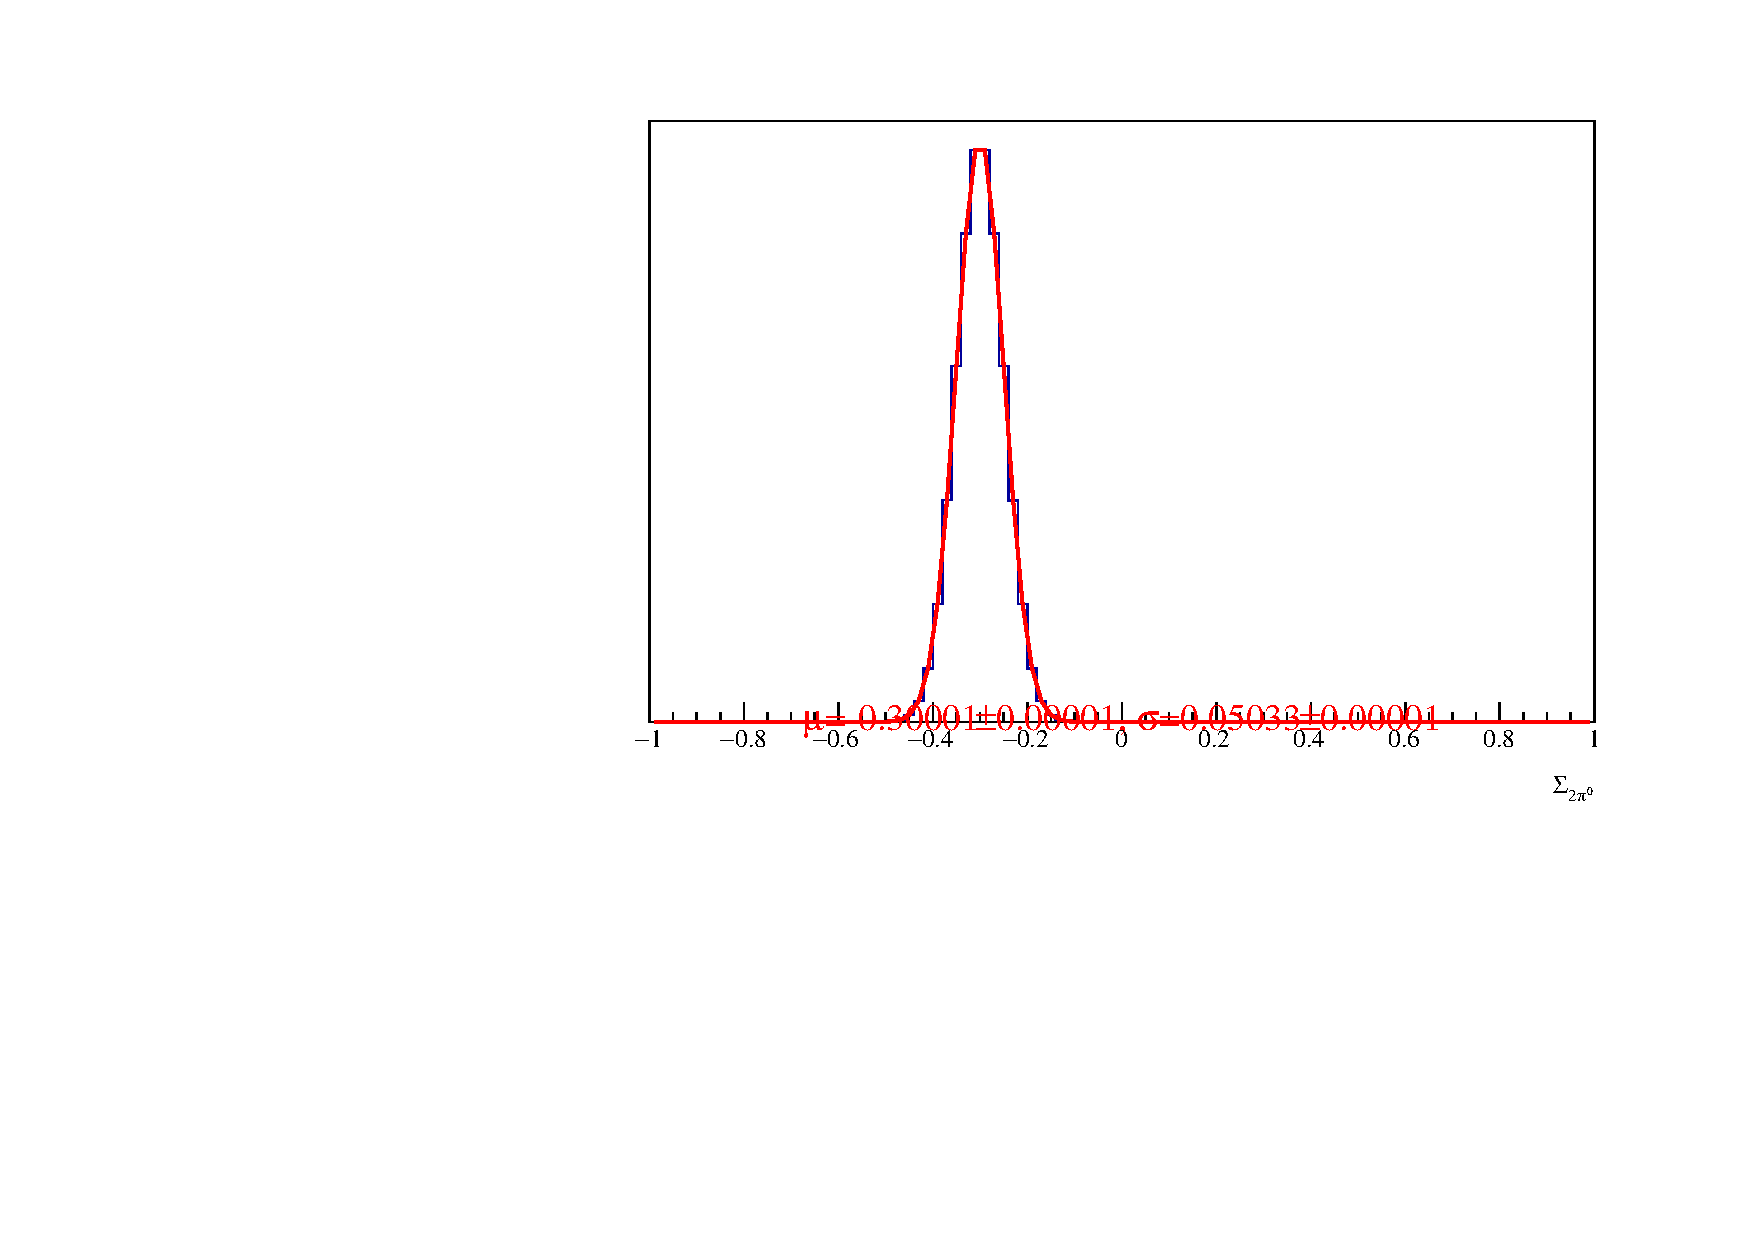
\includegraphics[width=.49\linewidth]{../../bayes/etap_event_based_fit/plots/combined2pi0_post_add_raw.pdf}
	
\end{frame}
\begin{frame}{Considering background contributions}
	Also, likelihood pool combination of posteriors again works nicely
	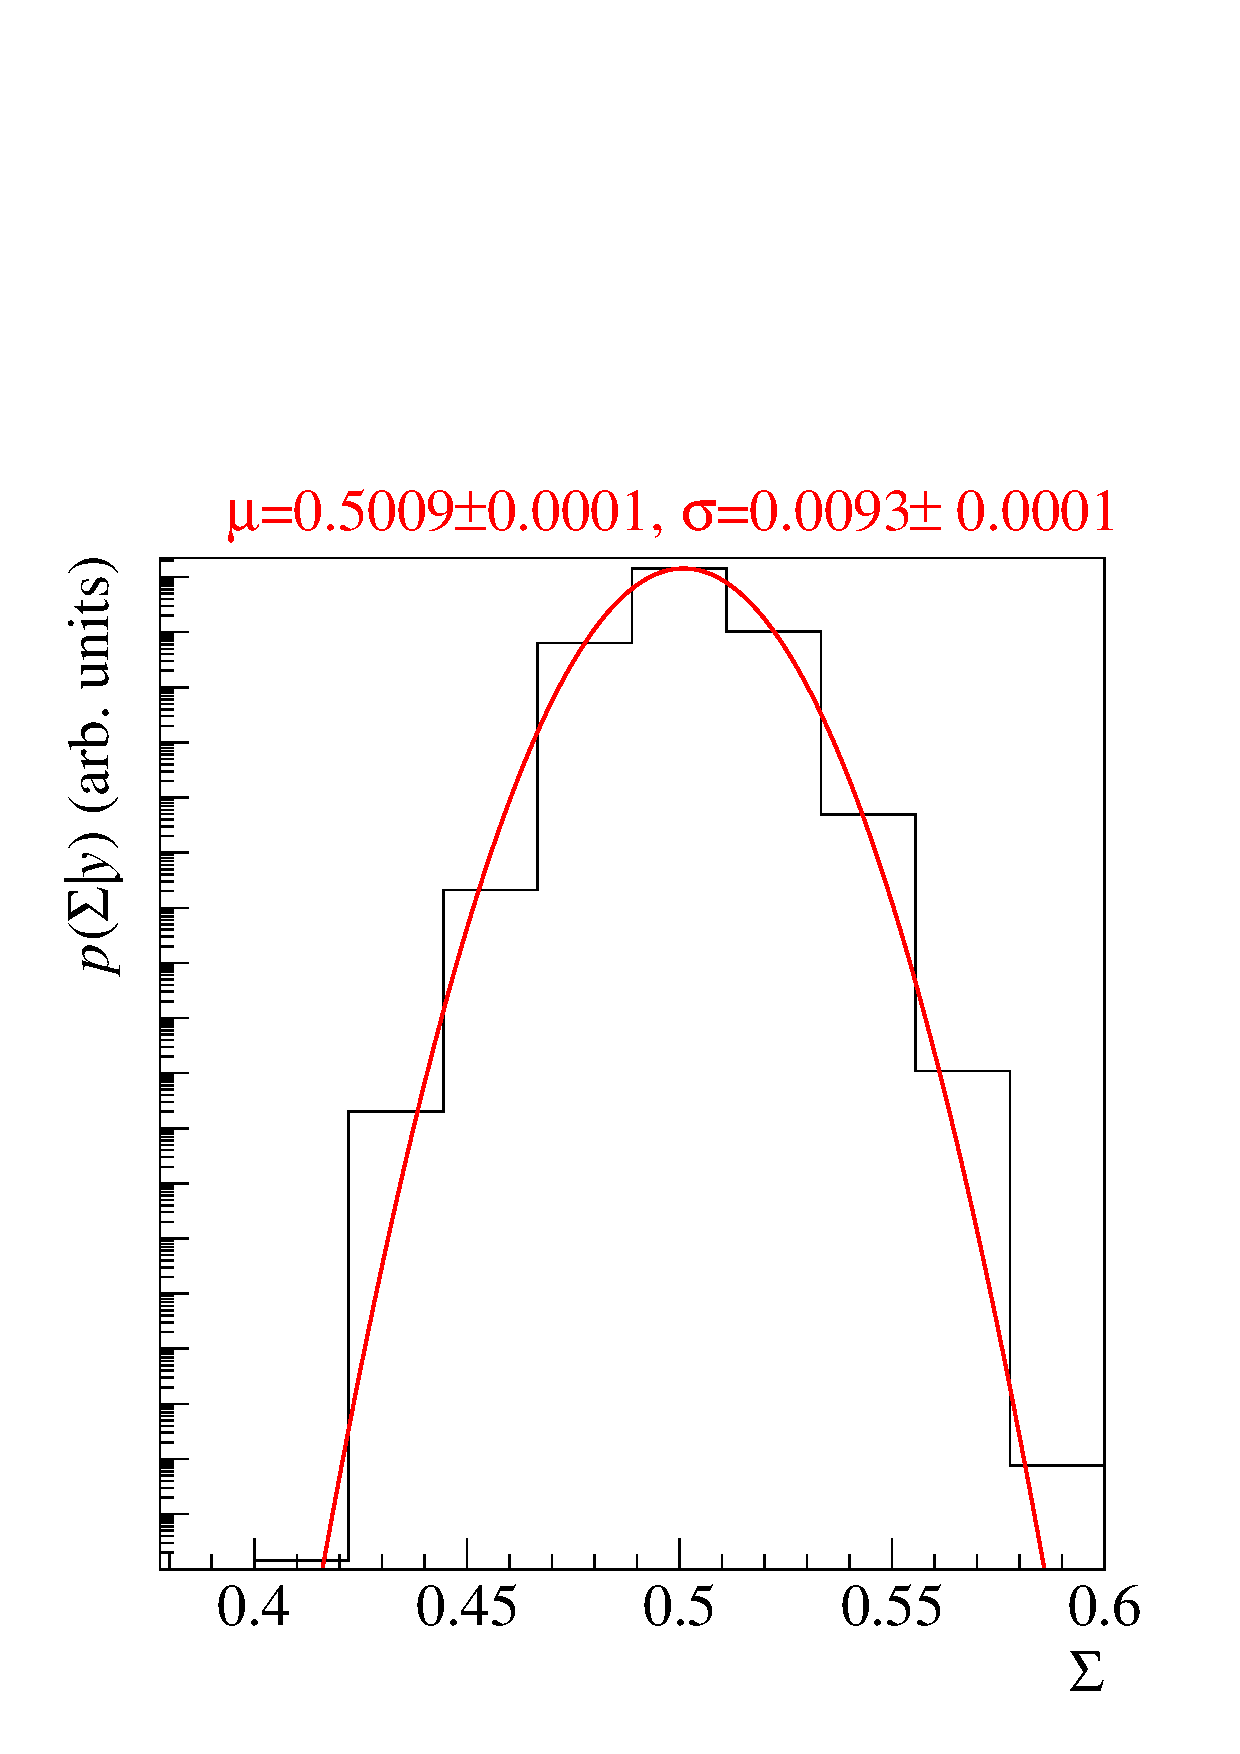
\includegraphics[width=.7\linewidth]{../../bayes/etap_event_based_fit/plots/combined_post_mul.pdf}		
\end{frame}
\begin{frame}{Results}
	\centering
	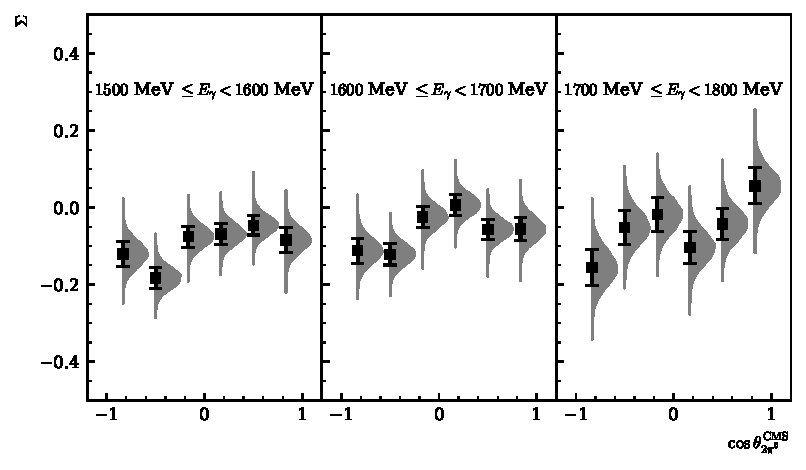
\includegraphics[width=.7\linewidth]{../../bayes/etap_event_based_fit/plots/sigma_2pi0.pdf}
\end{frame}
\begin{frame}{Results}
	\centering
	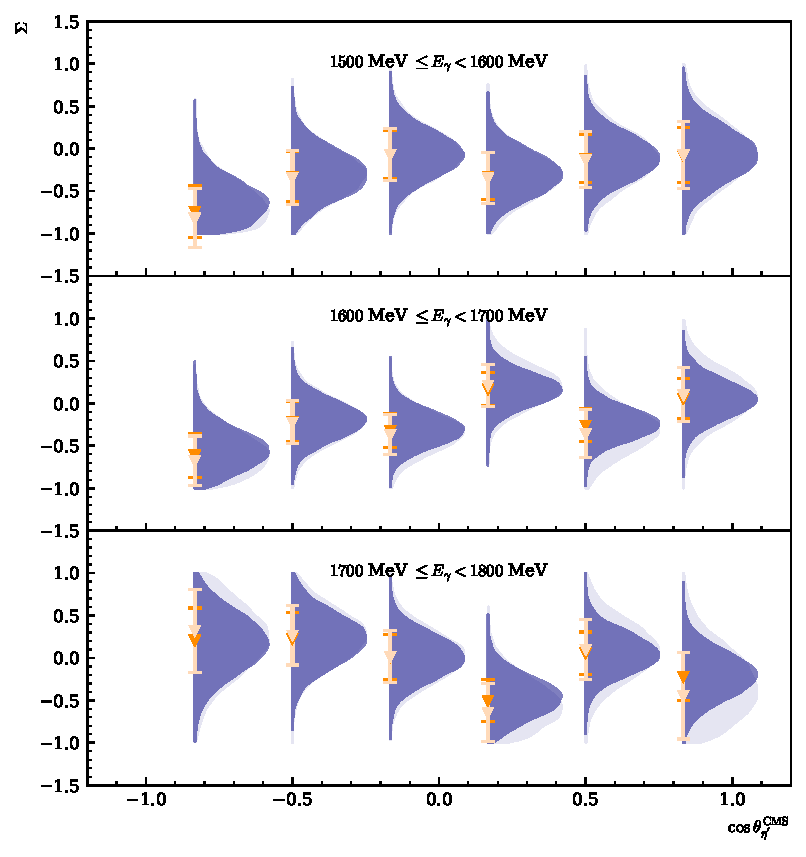
\includegraphics[width=.7\linewidth]{../../bayes/etap_event_based_fit/plots/sigma_etap.pdf}
\end{frame}
\end{document}
